% !TEX root = ..\thesis.tex

\chapter{MÔ HÌNH HỆ THỐNG}
% vẽ sơ đồ hệ thống

Mô hình tổng quan của đề tài hình \ref{fig:general_chart}
\begin{figure}[H]
    \centering
    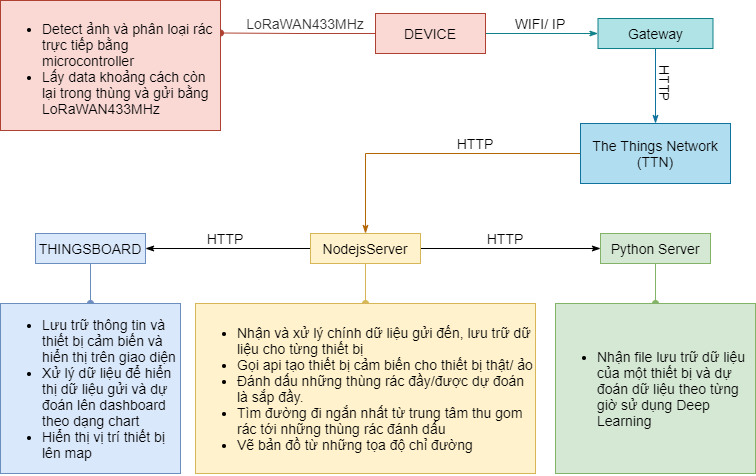
\includegraphics[width=\textwidth]{images/general_chart.png}
    \caption{Mô hình tổng quan}
    \label{fig:general_chart}
\end{figure}
Ở mô hình tổng quan đề tài, chúng tôi chia làm 2 phần, về thiết bị và về server.

\begin{itemize}
    \item Về thiết bị, chúng tôi gắn 2 loại board và 3 ultrasonic sensor, 1 servo vào thùng rác để thực hiện 2 mục đích khác nhau, cụ thể:
        \begin{itemize}
            \item ESP32 camera AI Thinker, dùng vào mục đích chụp ảnh và phục vụ chức năng phân loại rác thải.
            \item  ESP32 Lora heltec, dùng trong mục đích thu thập data và gửi data cho server bằng công nghệ LoRaWAN.
            \item 2 Ultrasonic sensor thực hiện nhiệm vụ đo độ dài khoảng trống còn lại trong thùng rác. Và 1 Ultrasonic sensor có nhiệm vụ phát hiện có rác trong thùng để camera được kích hoạt. 1 servo để tác động làm mặt đựng rác quay trái hoặc quay phải ứng với mục đích phân loại rác thải tái chế hay không tái chế.
        \end{itemize}

    \item Về server, sử dụng Nodejs và Flask làm server cung cấp API, Thingsboard để làm giao diện hiển thị và một số server thứ ba khác, chức năng được mô tả cụ thể như sau:
        \begin{itemize}
            \item Nodejs Server là server nhận và xử lý chính dữ liệu, lưu trữ dữ liệu cho từng thùng rác. Từ đó, sử dụng dữ liệu để hiển thị, dự đoán và tìm đường đi tối ưu nhất để thu gom rác.
            \item Flask Server là server sử dụng Deep Learning để dự đoán dữ liệu được gửi từ Nodejs Server.
            \item Thingsboard là giao diện lưu trữ thông tin thùng rác, hiển thị dữ liệu theo nhiều dạng và vẽ đường đi trên bản đồ.
            \item Ngoài ra, còn sử dụng Thingsboard server hỗ trợ API thao tác đến Thingsboard và Mapbox server hỗ trợ API liên quan đến địa lý và đường đi.
        \end{itemize}
   

\end{itemize}


Hình \ref{fig:chart_smartbin} mô tả chi tiết về cấu tạo của thùng rác, và các thức hoạt động của 2 loại board được gắn bên trong thùng. 
\begin{figure}[H]
    \centering
    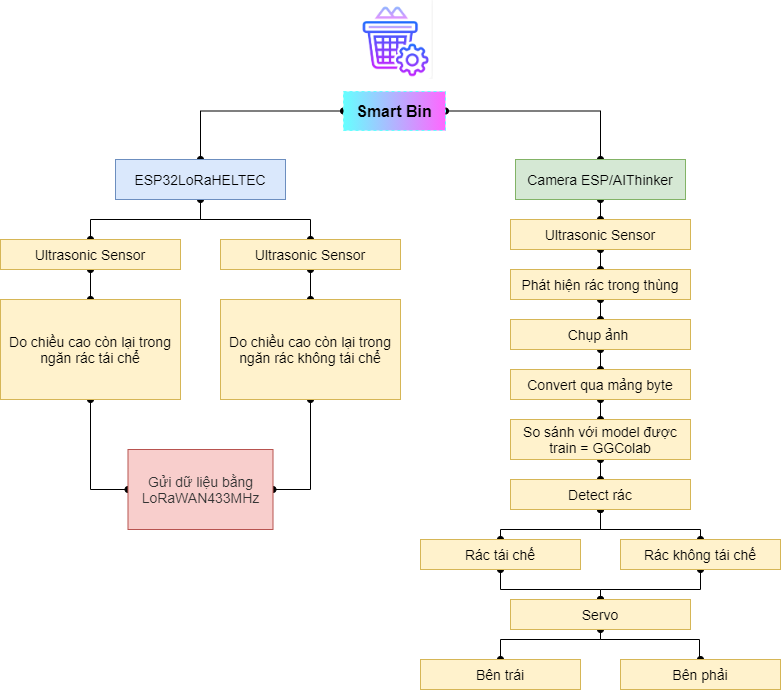
\includegraphics[width=\textwidth]{images/Chart_smartbin.png}
    \caption{Mô hình device}
    \label{fig:chart_smartbin}
\end{figure}

Như đã nói ở sơ đồ \ref{fig:general_chart}, Smart bin sẽ bao gồm 2 board, hoạt động cụ thể của chúng như sau:
\begin{itemize}
    \item Phân loại rác (ESP32Cam AI Thinker): Phía trong mặt trên của thùng rác được gắn 1 hộp thiết bị, bao gồm mạch ESP32Cam AI Thinker và 1 ultrasonic sensor.
    \begin{enumerate}
        \item Khi bỏ rác vào thùng, rác sẽ làm cho chiều cao của thùng thay đổi, cụ thể là khoảng cách từ mặt trên bên trong của thùng đến phần tiếp xúc của rác sẽ giảm. Từ đó, đáp ứng điều kiện để kích hoạt camera chụp ảnh.
        \item Camera chụp ảnh.
        \item Hình ảnh đã chụp được mạch thực hiện thao tác convert qua 1 mảng byte.
        \item Model detec ảnh đã được train từ Google Colab và đưa vào mạch cũng là 1 mảng byte. Nên mạch tiến hành so sánh 2 mảng byte đó và đưa ra kết quả detec.
        \item Sau khi có kết quả detec loại rác, mạch sẽ xét điều kiện xem loại rác đã được detec(glass/metal/plastic/cardboard/paper/other trash) thuộc loại rác: Tái tế hay Không tái chế.
        \item Sau khi có kết quả loại rác là "tái chế" hay " Không tái chế" thì mạch tiếp tục xét điều kiện:
        \begin{enumerate}
            \item Nếu rác thuộc loại "tái chế": servo sẽ quay 180 độ để làm rác rớt vào ngăn bên phải.
            \item Nếu rác thuộc loại "tái chế": servo sẽ quay 0 độ để làm rác rớt vào ngăn bên trái.
        \end{enumerate} 
    \end{enumerate}
    \item ESP32 Lora heltec, dùng trong mục đích thu thập data và gửi data cho server bằng công nghệ LoRaWAN. Bên trong thùng rác được thiết kế 2 ngăn, bên phải chứa rác không tái chế, bên phải chứa rác tái chế. Mỗi ngăn được gắn 1 ultrasonic sensor để thu thập dữ liệu về khoảng trống còn lại trong ngăn chứa rác, từ đó ESP32 Lora heltec sẽ gửi dữ liệu đến backend bằng công nghệ LoRaWAN.
\end{itemize}

Mô hình server từ bước khởi tạo đến gửi dữ liệu được vẽ ở hình \ref{fig:chart_server1} và được mô tả chi tiết như sau:
\begin{figure}[H]
    \centering
    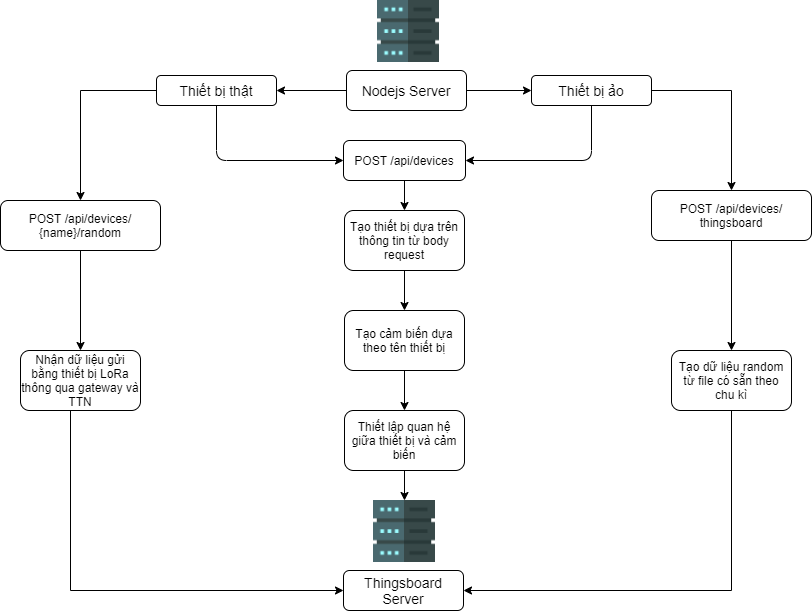
\includegraphics[width=\textwidth]{images/Khanh/Nodejs/Chart_server1.png}
    \caption{Mô hình server từ bước khởi tạo đến gửi dữ liệu}
    \label{fig:chart_server1}
\end{figure}

Chức năng chính của Nodejs Server là cung cấp API xử lý dữ liệu cho hai đối tượng chính là thùng rác thật và thùng rác ảo.
\begin{itemize}
    \item POST /api/devices: Hỗ trợ tạo thùng rác và các cảm biến liên quan bằng cách gửi request body bao gồm các thông số như tên, chiều cao, tọa độ ,... và tự động lưu vào database Thingsboard và cuối cùng là hiển thị trên dashboard. Thao tác này có thể thực hiện thủ công trên giao diện hoặc tự động thông qua API này.
    \item POST /api/TTN/telemetry: Nhận và xử lý dữ liệu được gửi từ các thùng rác thật thông qua gateway và TTN, format của dữ liệu bao gồm thông tin thùng rác và dữ liệu cảm biến. Dữ liệu được lưu vào file csv để dự đoán và được đưa lên Thingsboard để hiển thị trên dashboard.
    \item POST /api/devices/\{name\}/random: Tạo dữ liệu ngẫu nhiên cho thùng rác ảo với tên là \{name\} và được xử lý theo format dữ liệu giống với thiết bị thật. Dữ liệu được lưu vào file csv để dự đoán và được đưa lên Thingsboard để hiển thị trên dashboard.
\end{itemize}

Mô hình server từ sau bước gửi dữ liệu đến xử lý bản đồ được vẽ ở hình \ref{fig:chart_server2} và được mô tả chi tiết như sau:
\begin{figure}[H]
    \centering
    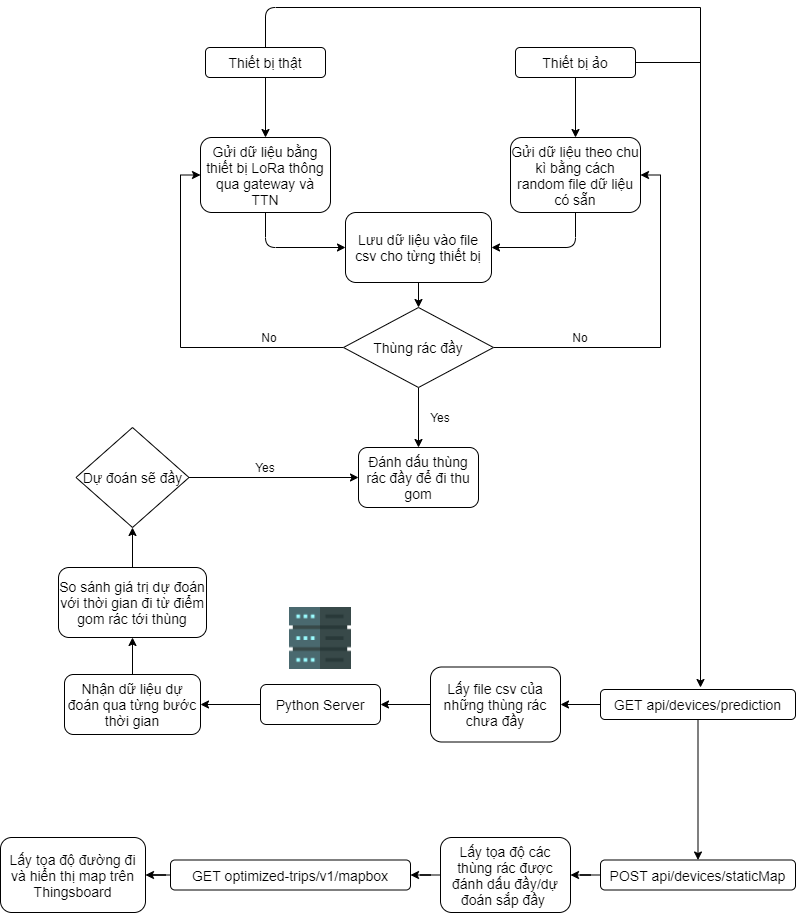
\includegraphics[width=\textwidth]{images/Khanh/Nodejs/Chart_server2.png}
    \caption{Mô hình server từ bước gửi dữ liệu đến xử lý bản đồ}
    \label{fig:chart_server2}
\end{figure}
Dữ liệu gửi tới sẽ được lưu trữ vào file csv cho đến khi thùng rác đầy, khi đó file csv sẽ ngưng ở giá trị lớn nhất và đợi đến khi nào thùng rác được gom sẽ tiếp tục nhận dữ liệu. Và khi thùng rác đầy, sẽ được đưa qua danh sách các thùng rác đầy để được đi thu gom.

Ngoài ra, Nodejs còn cung cấp 2 API gửi dữ liệu tiên đoán và tìm đường đi tối ưu cho cả 2 thiết bị thật và ảo:
\begin{itemize}
    \item GET api/devices/prediction: Đưa tất cả file csv dữ liệu của các thùng rác chưa đầy qua bên Python Server để xử lý dữ đoán dữ liệu qua các bước thời gian tiếp. Kết quả sẽ được trả về Nodejs Server, được so với thời gian di chuyển tử nơi gom rác đến thùng rác để chọn giá trị thích hợp và so với chiều cao thùng. Nếu giá trị lớn hơn 90\% thùng thì thùng đó sẽ được đưa vào danh sách thùng rác đầy.
    \item GET api/devices/staticMap: Lấy tất cả tọa độ trong danh sách thùng rác đầy và đưa qua API của Mapbox để vẽ ra đường đi tối ưu nhất để gom các thùng rác. Kết quả trả về là một mảng các tọa độ đường đi, sau đó được đưa lên Thingsboard để hiển thị trên bản đồ.
\end{itemize}

